\section{Methodology}
\label{sec:workflow}

\begin{figure*}[t]
    \centering
    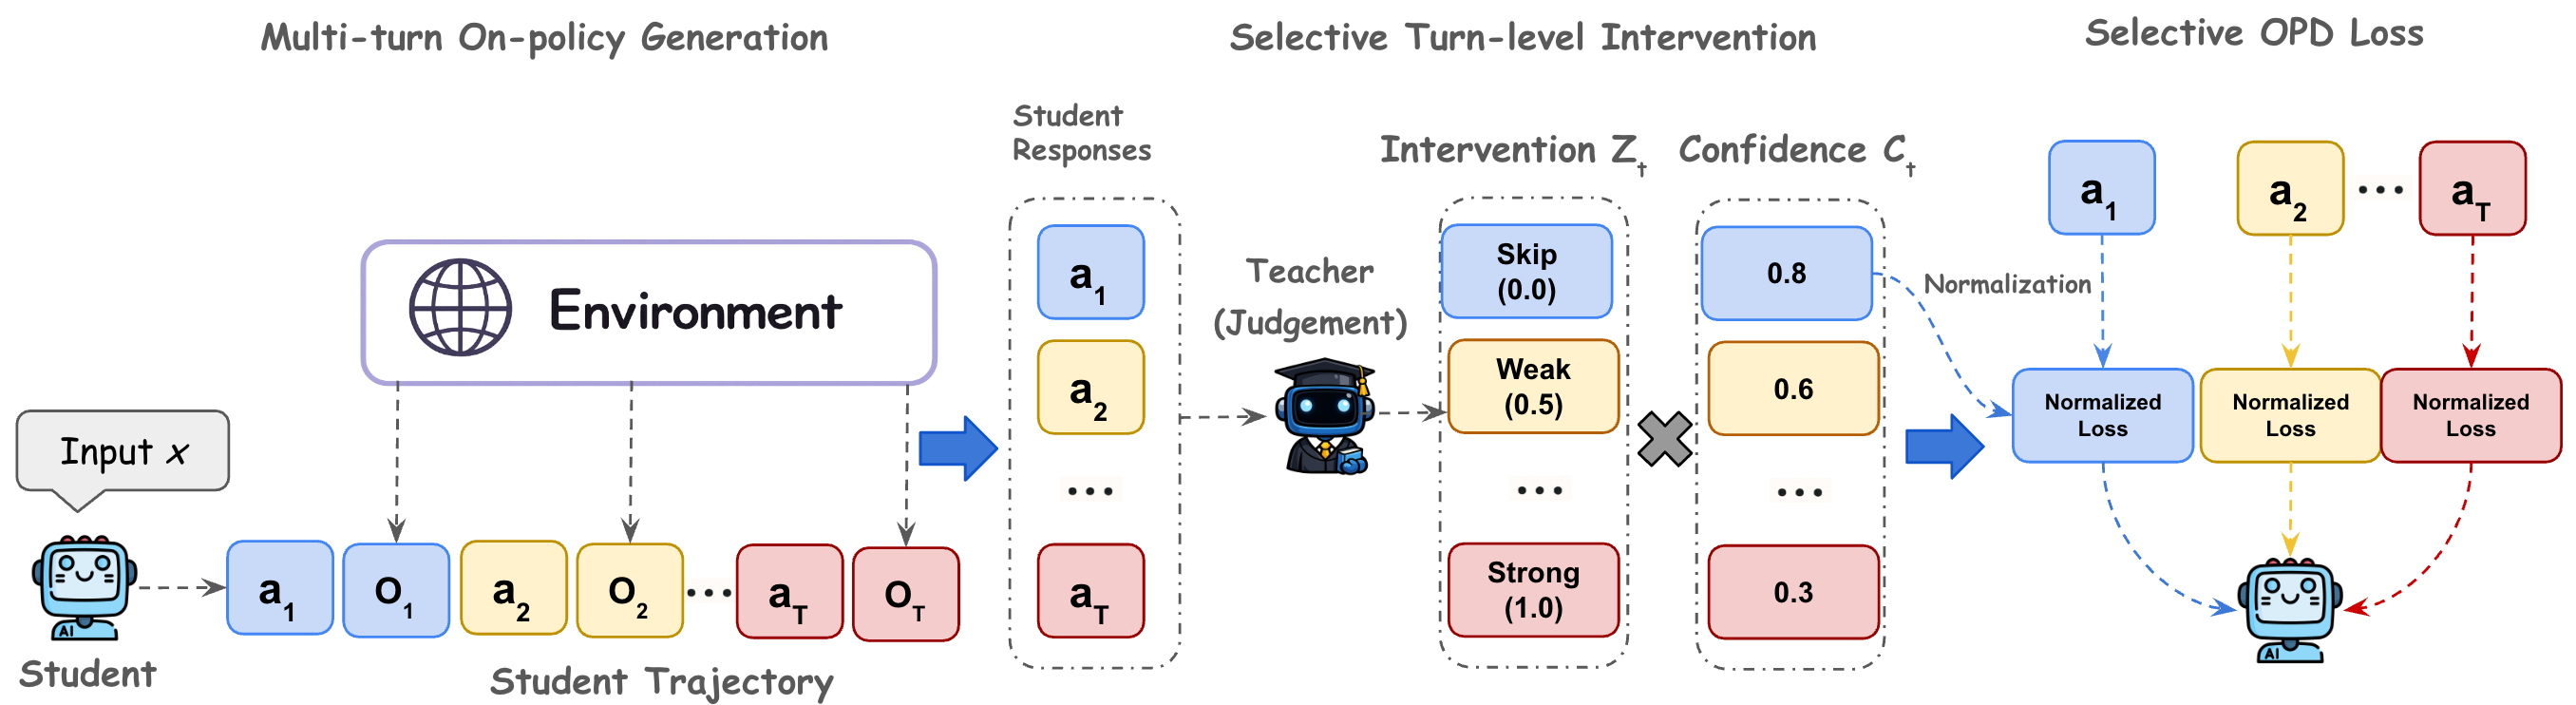
\includegraphics[width=\textwidth]{figure/diagram.png}
    \caption{
    Overview of \ours{}.
    %
    The student first performs multi-turn on-policy generation by interacting with the environment, producing a trajectory segmented into alternating actions and observations.
    %
    For each student turn, \ours{} uses environment feedback and teacher judgment to determine whether the response should be skipped or intervened on, and combines this intervention decision with the teacher confidence score.
    %
    The resulting selective weight modulates the OPD loss for each turn, so teacher supervision is applied more strongly when intervention is needed and the teacher signal is reliable.
    }
    \label{fig:our_framework}
\end{figure*}


\subsection{Preliminaries}

\paragraph{Multi-turn Agent Interaction.}
We consider a multi-turn agent interacting with an external environment over a sequence of action steps.
%
At turn $t$, the agent receives an observation $o_t$ and conditions on the full interaction history $h_t=(o_0,a_0,\ldots,o_{t-1},a_{t-1},o_t)$, where $a_i$ denotes the model response at turn $i$.
%
The response $a_t$ may include natural language reasoning, tool-use arguments, and an executable action.
%
After the executable part of $a_t$ is submitted to the environment, the environment returns the next observation $o_{t+1}\sim\mathcal{E}(\cdot\mid h_t,a_t)$.
%
A complete trajectory is $\tau=(h_0,a_0,\ldots,h_{T-1},a_{T-1})$, which terminates when a termination action is taken or when the maximum horizon $T$ is reached.
%
This dependency distinguishes multi-turn agent learning from single-turn generation: an early mistake can alter the environment state and affect all subsequent observations.

\paragraph{Multi-turn On-Policy Distillation.}
Let $\pi_\theta$ denote the student policy and $\pi_\phi$ denote the teacher policy.
%
In multi-turn OPD, trajectories are sampled from the student policy, i.e., $a_t\sim\pi_\theta(\cdot\mid h_t)$.
%
The teacher then provides supervision on these student-induced states.
%
We write the standard multi-turn OPD objective as
\begin{equation}
\label{eq:opd_objective}
\resizebox{0.96\columnwidth}{!}{$
\displaystyle
\mathcal{L}_{\mathrm{OPD}}
=
\mathbb{E}_{\tau\sim\pi_\theta}
\sum_{t=0}^{T-1}
\ell_{\mathrm{OPD}}(h_t),
\quad
\ell_{\mathrm{OPD}}(h_t)
=
D_{\mathrm{KL}}
\bigl(
\pi_\theta(\cdot\mid h_t)
\Vert
\pi_\phi(\cdot\mid h_t)
\bigr).
$}
\end{equation}
%
The student is therefore trained on its own state distribution, allowing the teacher to supervise states that arise from the student's behavior rather than only from ideal teacher-generated trajectories.

However, applying OPD uniformly to every turn in a multi-turn trajectory can be suboptimal.
%
Early student errors may alter future observations and push later histories away from the teacher's reliable state distribution, making subsequent supervision less dependable.
%
Meanwhile, token-level OPD can be brittle when teacher and student policies assign probability mass to different but semantically valid continuations, or when dense alignment reinforces local degeneracies such as repeated thoughts or actions.
%
These issues motivate a selective mechanism that decides when teacher distillation should be applied and how strongly the resulting signal should be trusted.

\subsection{\ours{}}
\label{sec:method}

The limitations of dense multi-turn OPD suggest that teacher supervision should be applied selectively rather than uniformly across all turns.
%
Standard OPD treats a student trajectory as a flat sequence of tokens and applies teacher distillation everywhere, which makes training sensitive to token-level mismatch even when the student response is semantically acceptable.
%
Multi-turn interaction provides a natural way to move beyond this flat token-level view: the trajectory is already segmented by environment feedback, where each turn produces a response $a_t$, receives an observation, and transitions to a new history $h_{t+1}$.
%
This turn structure allows the teacher to critique larger units of behavior and decide whether token-level distillation is needed for the current student response.

At the same time, teacher supervision should not be trusted uniformly across the trajectory.
%
Because student errors can compound over multiple turns, later histories may drift away from the teacher's reliable state distribution, making token-level supervision less dependable.
%
Motivated by these observations, and illustrated in \figref{fig:our_framework}, we propose \ours{}, a selective intervention framework for multi-turn OPD.
%
For each turn, \ours{} observes the environment feedback and uses teacher judgment to decide whether the current student response should be skipped or intervened on.
%
It then weights the token-level OPD objective by the teacher's predictive confidence, so supervision is strongest when intervention is needed and the teacher signal is reliable.
%
Finally, \ours{} applies vanilla-scale normalization to preserve the overall loss scale of standard OPD while retaining selective turn-level weighting.
%
The full training procedure is presented in Algorithm~\ref{alg:sl_opd} in \appref{sec:implementation_details}.

\subsection{Turn-Level Intervention}
\label{sec:method_intervention}

To obtain turn-level supervision without a task verifier, we introduce a discrete intervention label $z_t\in\{\textsc{Skip},\textsc{Weak},\textsc{Strong}\}$.
%
Each label is mapped to a scalar intervention weight:
\begin{equation}
\label{eq:intervention_weight}
i_t =
\begin{cases}
0, & z_t=\textsc{Skip},\\
\alpha, & z_t=\textsc{Weak},\\
1, & z_t=\textsc{Strong},
\end{cases}
\end{equation}
where $\alpha\in(0,1)$ controls the strength of weak intervention.
%
The \textsc{Skip} label suppresses OPD at the current turn, \textsc{Weak} applies partial teacher supervision, and \textsc{Strong} applies full teacher supervision.

We assign $z_t$ through a two-stage verifier-free procedure.
%
First, we inspect the environment feedback for deterministic interaction failures.
%
If the student response produces a clearly invalid transition, such as a failed tool call, missing executable action, or other environment-detectable execution failure, we directly set $z_t=\textsc{Strong}$ and $i_t=1$.
%
These cases do not require semantic judgment from the teacher, since the environment already indicates that the current response should be corrected.
%
For all remaining turns, where the response is executable but its quality is ambiguous, we query the teacher with an intervention-evaluation prompt.
%
Given the interaction history $h_t$, the student response $a_t$, and the available environment feedback, the teacher classifies the turn into exactly one of $\{\textsc{Skip},\textsc{Weak},\textsc{Strong}\}$.
%
Intuitively, \textsc{Skip} is used when the response is acceptable or when multiple strategies are plausible; \textsc{Weak} is used when the response may be suboptimal but the teacher is not fully certain; and \textsc{Strong} is used when the response is clearly detrimental and teacher correction is necessary.
%
Prompt details are provided in \appref{sec:appendix_prompts}.

\subsection{Teacher Confidence Weighting}

The intervention label determines whether teacher supervision is needed at a given turn.
%
However, even when intervention is needed, the teacher's token-level supervision may not always be reliable.
%
Due to compounding errors in multi-turn interaction, the student may enter histories that deviate from the teacher's reliable state distribution.
%
In such cases, the teacher may still recommend intervention, but its predictive distribution can be uncertain.
%
We therefore introduce a confidence score $c_t$ to measure how decisive the teacher is at turn $t$.

For each token position $j$ in the student response $a_t$, let $p^\star_{t,j}=\max_v\pi_\phi(v\mid h_t,a_{t,<j})$ denote the teacher's top-1 probability.
%
We define the turn-level confidence score and final selective weight as
\begin{equation}
\label{eq:confidence_weight}
c_t =
\frac{1}{|a_t|}
\sum_{j=1}^{|a_t|}
p^\star_{t,j},
\qquad
s_t = i_t c_t .
\end{equation}
%
A sharp teacher distribution yields a high $c_t$, indicating that the teacher is confident about the token-level supervision for this turn.
%
Conversely, a flat distribution yields a low $c_t$, indicating that the teacher itself is uncertain and that the resulting distillation signal should be weakened.
%
The same weight $s_t$ is applied uniformly to all token-level OPD terms within turn $t$.
%
Since $p^\star_{t,j}$ is obtained from the same teacher distribution used for the standard distillation loss, computing $c_t$ introduces no additional teacher forward passes beyond the intervention query.

\subsection{Vanilla-Scale Normalization}

The selective weight $s_t\in[0,1]$ controls how strongly teacher supervision is applied at turn $t$.
%
However, directly multiplying the OPD loss by $s_t$ also reduces the overall gradient magnitude relative to vanilla OPD.
%
This makes it difficult to distinguish the effect of selective supervision from the effect of training with a smaller effective learning rate.
%
To isolate the contribution of selective weighting, we normalize the loss scale within each batch.

Let $\ell_{\mathrm{OPD}}(h_t,a_t)$ denote the token-level OPD loss for turn $t$, and let $N$ denote the total number of student tokens in the trajectory or batch.
%
We define the normalized selective OPD objective as
\begin{equation}
\label{eq:selective_loss}
\begin{aligned}
\mathcal{L}_{\ours}
&=
Z\sum_{t}
s_t\ell_{\mathrm{OPD}}(h_t,a_t), \\
Z
&=
\frac{N}{
\max\!\left(
\sum_{t}s_t|a_t|,
\epsilon
\right)} .
\end{aligned}
\end{equation}
%
Here, $|a_t|$ is the number of student tokens in turn $t$, and $\epsilon$ is a small constant for numerical stability.
%
This normalization keeps the average effective token weight close to one, matching the scale of vanilla OPD while preserving the relative turn-level weighting induced by $s_t$.
%
As a result, \ours{} provides a verifier-free turn-level supervision policy that selectively reallocates teacher supervision without merely reducing the overall training signal.

\subsection{Analysis of Selective Weighting}
\label{sec:theory}

We provide an analysis to clarify the role of selective weighting in \ours{}.
%
Our goal is not to prove that the teacher intervention gate is always correct, but to formalize two intuitions: selective weights suppress noisy supervision from low-reliability turns, and the quality of selective OPD depends on how well its weights approximate an ideal intervention policy.
%
Let $\ell_t(\theta)$ denote the per-turn OPD loss at turn $t$, and let $s_t=i_tc_t\in[0,1]$ be the selective weight.
%
The normalized objective follows \eqref{eq:selective_loss}, with $\ell_{\mathrm{OPD}}(h_t,a_t)$ replaced by $\ell_t(\theta)$.

\paragraph{Selective suppression of noisy supervision.}
Assume that the observed per-turn OPD loss decomposes as $\ell_t(\theta)=\ell_t^\star(\theta)+\xi_t$, where $\ell_t^\star$ is the ideal supervision loss and $\xi_t$ is zero-mean noise caused by teacher uncertainty, token-level mismatch, or off-distribution histories.
%
Assume $\mathrm{Var}[\xi_t]\leq\sigma_t^2$.
%
For a fixed batch, define the normalized effective weight as $\widetilde{s}_t=Zs_t$.

\begin{proposition}[Relative Suppression of Noisy Supervision]
\label{prop:relative_suppression}
The variance contribution of turn $t$ to the noisy component of the normalized selective objective is bounded by
\begin{equation}
\label{eq:noise_bound}
\mathrm{Var}[\widetilde{s}_t\xi_t]
\leq
\widetilde{s}_t^2\sigma_t^2 .
\end{equation}
Moreover, if two turns $p$ and $q$ satisfy $s_p\leq\gamma s_q$ for some $\gamma<1$, then their per-unit-noise contributions satisfy $\widetilde{s}_p^2/\widetilde{s}_q^2\leq\gamma^2$.
\end{proposition}

This proposition does not claim that the total variance of \ours{} is always smaller than that of vanilla OPD.
%
Because vanilla-scale normalization may produce $Z>1$, the absolute variance of the normalized objective can increase in some batches.
%
Instead, the result shows that the relative suppression induced by $s_t$ is preserved after normalization.
%
When the intervention mechanism assigns smaller weights to unnecessary or unreliable turns, their noisy teacher gradients are reduced relative to turns where intervention is needed and the teacher signal is confident.
%
The proof is provided in \appref{sec:appendix_theory}.

\paragraph{Connection to oracle intervention.}
An ideal selective OPD objective would supervise exactly the turns where teacher correction is useful.
%
Let $m_t^\star\in\{0,1\}$ denote this unobserved oracle intervention indicator, where $m_t^\star=1$ means that turn $t$ should receive teacher supervision and $m_t^\star=0$ means that it should be skipped.
%
The oracle objective is $\mathcal{L}_{\mathrm{oracle}}(\theta)=\sum_{t=0}^{T-1}m_t^\star\ell_t(\theta)$.
%
Our method replaces this binary oracle mask with the verifier-free soft weight $s_t=i_tc_t$.

\begin{proposition}[Approximation Error of Selective Intervention]
\label{prop:oracle_approx}
If the per-turn loss is bounded as $0\leq\ell_t(\theta)\leq B$, then
\begin{equation}
\label{eq:oracle_bound}
\left|
\sum_{t=0}^{T-1}
(s_t-m_t^\star)\ell_t(\theta)
\right|
\leq
B\sum_{t=0}^{T-1}
|s_t-m_t^\star| .
\end{equation}
\end{proposition}

This bound is not a guarantee that \ours{} recovers the oracle mask.
%
Rather, it makes explicit that the gap to oracle selective supervision is controlled by the quality of the intervention weights.
%
In \ours{}, deterministic environment failures provide high-precision positive intervention signals, teacher judgment approximates the oracle decision for executable but ambiguous turns, and teacher confidence softens the weight when token-level supervision is uncertain.
%
The proof is provided in \appref{sec:appendix_theory}.